\documentclass[journal]{IEEEtran}
\usepackage{cmap}
\usepackage{amsmath}
\usepackage{amsfonts}
\usepackage{subfigure}
\usepackage[final]{graphicx}
\usepackage{graphics,picture}
\usepackage[boxed,noline]{algorithm2e}
\usepackage{mathrsfs}
\usepackage{cases}
\usepackage{bm, comment,color,amssymb}
\usepackage{cite,epstopdf}
\renewcommand{\thefootnote}{\arabic{footnote}}
\newcommand{\trace}{\mathop{\mathrm{Tr}}}%\trace
\newcommand{\vectorize}{\mathop{\mathrm{vec}}}%\vectorization

\begin{document}
	
\title{Blockchain-based Distributed Dynamic Spectrum Optmization}
	
\author{Miao Jiang, Yiqing Li, Qi Zhang, \emph{Member}, \emph{IEEE}, and Jiayin Qin

\thanks{This work was supported in part by the National Natural Science Foundation of China under Grant 61672549 and Grant 61472458, and in part by the Guangzhou Science and Technology Program under Grant 201607010098 and Grant 201804010445.

M. Jiang, Y. Li, and Q. Zhang are with the School of Electronics and Information Technology, Sun Yat-sen University, Guangzhou 510006, Guangdong, China (e-mail: jmiao@mail2.sysu.edu.cn, liyiq5@mail2.sysu.edu.cn, zhqi26@mail.sysu.edu.cn). J. Qin is with the School of Electronics and
Information Technology, Sun Yat-sen University, Guangzhou 510006, Guangdong,  China, and also with the Xinhua College, Sun Yat-sen University, Guangzhou 510520, Guangdong, China (e-mail: issqjy@mail.sysu.edu.cn). }
}% <-this % stops a space
	
	
\markboth{Submitted to IEEE Transactions on Vehicular Technology}
{Jiang \MakeLowercase{\textit{et al.}}: Blockchain-based Distributed Dynamic Spectrum Optmization}
	
\maketitle
\begin{abstract}
In this paper, we investigate a two-stage spectrum leasing framework in the virtualized wireless network (VWN). During the first stage, the mobile network operator (MNO) leases spectrum to $N$ mobile virtual network operators (MVNOs). We focus on the spectrum and power allocation factors design which minimizes the total transmit power at MVNOs. The original optimization problem is hard to be solved due to the complex integration expressions in the constraints. We first employ half-range Gauss-Hermite Quadrature (HR-GHQ) to simplify the optimization problem. Then, we propose a blockchain-based spectrum management scheme combined with alternative direction method of multipliers (ADMM) to obtain the global optimal solutions. Such a distributed optimization scheme based on blockchain can ensure security and transparency during the spectrum management. During the second stage, each MVNO dynamically allocates the spectrum that has already been rent from MNO to mobile users (MUs). We derive closed-form expressions for the optimal spectrum and power allocation for each MVNO. Simulation results are provided to validate the effectiveness of our proposed algorithm.
\end{abstract}
\begin{IEEEkeywords} Virtualized wireless network (VWN), blockchain, alternating direction method of multipliers (ADMM), convex optimization, spectrum management.
\end{IEEEkeywords}
\IEEEpeerreviewmaketitle
	
\section{introduction}
With the popularity of various smart phones, the dramatic traffic growth generated by wireless applications is undergoing an exponential growth in next generation 5G networks and beyond \cite{NPanwar,NAlFalahy}. Network densification is expected to increase by 1000 times ranging from macrocell to femtocell and the demands for radio spectrum resources are increasing unprecedentedly \cite{AYDing}. Therefore, we are facing a serious spectrum shortage problem. One of the reasons is that the spectrum system of access today has a binary quality, namely, either it is licensed or unlicensed \cite{JRosenworcel}. For an unlicensed mobile user (MU), it is not allowed to transmit even when the licensed part of the spectrum is idle, which results in underutilization of licensed spectrum in wireless communication. This phenomenon is not the result of physics and effective spectrum management is vitally important to solve this problem.

Wireless network virtualization (WNV) is a promising solution to improve the spectrum efficiency \cite{CLiang,LZhao,3GPP}. WNV can facilitate multiple network operators to share common resources, e.g., licensed spectrum. The virtualized wireless networks (VWNs) commonly consist of MNO (mobile network operator) and MVNO (mobile virtual network operator) \cite{RKokku}. The MNO owns the physical cellular infrastructure and radio resources, it executes the virtualization by leasing the isolated virtualized network resources to the MVNO. The MVNO leases the resources from the MNO and then assigns the resources to the MUs. The spectrum resources belong to one or more MNOs and are virtualized and spitted into slices. The MVNO utilizes the slices from MNOs depending on the quality-of-service (QoS) of MUs. Recently, WNV has attracted an increasing attention increasing attention from the research community \cite{XCostaPerez,MIKamel,MKalil,YXZhang1,YXZhang2}. In \cite{XCostaPerez}, an active sharing of physical infrastructure and the spectrum was introduced, where MNOs share the network resources and provide wholesale access to MVNOs, allowing them to provide voice and data services using part of the available resources. The work in \cite{MIKamel} introduced a novel scheme for slicing and scheduling for VWNs by developing an efficient resource allocation scheme. In \cite{MKalil}, an efficient low-complexity
scheme was proposed to virtualize the wireless resource blocks and
share them between MUs of multiple MNOs. The scheme aims to maximize the throughput
while fairness among MUs as well as MNOs. \cite{YXZhang1} proposed a two-stage spectrum leasing problem with the goal of maximizing $\alpha$-fair utility function by solving the optimal long-term and short-term leases jointly. A similar two-stage spectrum leasing problem was investigated in \cite{YXZhang2}, where the MVNO takes advantage of both the low cost of advance reservation and the flexibility of on-demand request to maximize the MVNO’s surplus problem.

All the above dynamic spectrum allocation schemes in VWNs can improve the usage of spectrum efficiently. While spectrum management in licensed bands has
mostly been controlled by responsible government agencies, the requirement of bringing market based reform in spectrum trading is being increasingly recognized to promote flexibility in radio spectrum use \cite{FBltr}. Thus, a central utility is needed to manage and record the usage of the spectrum as well as charge MUs for the spectrum occupation. However, following problems may arise in such a centralized utility: firstly, the overhead of management is quite high; secondly, the centralized structure is not robust to cyberattacks; thirdly, spectrum leasing fee is not transparent. Therefore, a smarter and more decentralized dynamic spectrum access technique, e.g., blockchain, is emerging.

Blockchain, which was invented by Satoshi Nakamoto in 2008, is an emerging technology to build consensus between disparate individuals \cite{SNakamoto}. The intuition is to solve the double-spending problem in the cryptocurrency bitcoin without the use of a trusted central utility. Blockchain consists of lists of blocks which are linked by hash algorithm. Each block includes collections of signatured transactions. A new block can be appended to the end of the current blockchain after solving a proof-of-work (PoW) puzzle which is to find a number whose hash value is less than the current target. PoW can create distributed consensus between all participants and solve the double-spend problem. The data on blockchain is shared and saved by all participants on peer-to-peer networks. All participants have right to access but cannot tamper the data on blockchain. The pillars of blockchain are state-of-the-art cryptography and PoW based distributed consensus mechanism. This kind of system may introduce some computational cost but can provide decentrality, security, transparency and robustness. The blockchain technologies have attracted remarkable interests and have been used in many areas extensively \cite{KGai,PKSharma,ZXiong,DBRawat,E. Munsing,KKotobi}. In \cite{KGai}, potential fusion of blockchains and cloud computing from the perspectives of secure data transfer and transparent data usage was investigated. To satisfy the rapid increase in the number and diversity
of smart phones connected to the Internet, a new distributed secure Internet of Things (IoT) network architecture named DistBlockNet was proposed in \cite{PKSharma}. The paper in \cite{ZXiong} investigated the price-based computing resource management in PoW based public blockchain networks to support offloading mining tasks intended for cloud/fog provider. In \cite{DBRawat}, the authors leveraged the blockchain based scheme for MVNOs to serve wireless users without sharing their
private information to anyone else
and enhance overall network coverage and capacity. By using blockchains and smart contracts, the work in \cite{E. Munsing} proposed a decentralized ADMM based optimal power flow (OPF) model for a microgrid. A blockchain based spectrum sharing scheme and a virtual cryptocurrency named Specoins was proposed in \cite{KKotobi}, which makes mobile users access the wireless channel dynamically in cognitive radio (CR) networks. However, to the best of our knowledge, the blockchain-based dynamic spectrum allocation combined with convex optimization in VWNs is still missing.

In this paper, we investigate a two-stage spectrum leasing framework in the virtualized wireless network (VWN). During the first stage, the mobile network operator (MNO) leases spectrum to $N$ mobile virtual network operators (MVNOs). We focus on the spectrum and power allocation factors design which minimizes the total transmit power at MVNOs. The original optimization problem is hard to be solved due to the complex integration expressions in the constraints. We first employ half-range Gauss-Hermite Quadrature (HR-GHQ) to simplify the optimization problem. Then, we propose a blockchain-based spectrum management scheme combined with alternative direction method of multipliers (ADMM) to obtain the global optimal solutions. Such a distributed optimization scheme based on blockchain can ensure security and transparency during the spectrum management. During the second stage, each MVNO dynamically allocates the spectrum that has already been rent from MNO to mobile users (MUs). We derive closed-form expressions for the optimal spectrum and power allocation for each MVNO. Simulation results are provided to validate the effectiveness of our proposed algorithm.

The remainder of the paper is organized as follows. The system model and problem formulation is described in Section II. Spectrum leasing and power allocation during the first stage are solved in Section III. Dynamic spectrum allocation and power allocation during the second stage are provided in Section IV. Section V provides simulation results to validate the effectiveness of our proposed scheme. At last, Section VI concludes this paper.

\emph{Notations}: Boldface lowercase letters denotes vectors. $\left(\cdot\right)^T$ denotes the transpose. $\left\|\cdot \right\|_1$ and $\left\|\cdot \right\|_2$ represent the $l_1$ and $l_2$ norm of a vector, respectively.
\section{System Model and Problem Formulation}
Consider a wireless communication system with one MNO and $N$ MVNOs. With wireless network virtualization operation, the whole communication processes are divided into two stages. MVNOs will first rent wireless spectrum from the MNO and then provide customized services to their MUs in their respective service cells. Particularly, we investigate an orthogonal multiple access downlink transmission scenario. Denote the bandwidth occupied by the $i$-th MVNO during the first transmission stage as $w_i$. Thus, we have
\begin{align}
\sum_{i = 1}^{N} w_i \leq W_{sum},
\end{align}
where the total bandwidth owned by MNO is $W_{sum}$ Hertz (Hz). In this paper, without loss of generality, we approximate the $i$-th transmission cell as a fixed circular region $\mathcal{D}(\mathbf{o}_i, r_i) \in \mathbb{R}^2$, where $r_i$ denotes the cell radius and $\mathbf{o}_i$ denotes the cell center. The $i$-th MVNO is located at the origin $\mathbf{o}_i$. The locations of MUs are modeled as a realization of a Poisson point process (PPP) with intensity $\lambda_i$ in the $i$-th cell. The locations of MUs associated with the $i$-th MVNO are denoted as $\mathcal{X}_i = \{\mathbf{x}_{ij} \in \mathbb{R}^2 | j = 1, \cdots, N_i\}$, where $N_i = \pi r_i^2 \lambda_i$ is the expected number of MUs in the $i$-th cell. Note that the user set $\mathcal{X}_i$ changes with arrivals, departure, and movements of MUs.

Suppose that transmitted signals are affected by both large-scale path loss and fast Rayleigh fading. Thus, the channel between the $j$-th MU and its associated $i$-th MVNO is denoted by $h_{ij} = \frac{g_{ij}}{\sqrt{1 + {\left\| \mathbf{x}_{ij} - \mathbf{o}_i \right\|}^\alpha}}$, where $\alpha$ denotes the path-loss decay factor  and $g_{ij}$ denotes the Rayleigh fading channel state information (CSI), i.e., $g_{ij}$ is a complex Gaussian random variable with zero mean and unit variance. The instantaneous data rate for the $j$-th MU in the $i$-th MVNO is given by
\begin{align}
	R_{ij} = b_{ij}\log_2\left(1 + \frac{q_{ij} \left|h_{ij} \right|^2 }{\Gamma b_{ij}\sigma_0}\right),
\end{align}
where $b_{ij}$ and $q_{ij}$ denotes the bandwidth and power of the $j$-th MU allocated by the $i$-th MVNO, respectively. $\Gamma$ denotes the SNR gap to the information theoretical channel capacity owing to the
non-ideal coding and modulation in practice \cite{JGDForney}. We assume that the power spectral densities of white noise at different MUs are equal and denoted as $n_0$.                  
\begin{figure}
	\centering
	\includegraphics[width=3.6in]{Pic.eps}
	\caption{Two-stage spectrum leasing network. During the first stage, MVNOs rent spectrum from an MNO based on the arrival rate and QoS of MUs. During the second stage, each MVNO allocates the obtained spectrum dynamically to a set of MUs.}
\end{figure}

The two-stage spectrum leasing processes are operated in two timescales, namely a period and a time slot. As shown in Fig. 1, the first stage is operated in a period and often measured in hours, where each MVNO rents wireless spectrum from a MNO. The second stage is operated in multiple time slots and often measured in milliseconds. Each period has multiple time slots. Wireless channel fading remains constant in a time slot but may change from one time slot to another. Notice that MVNOs will not release the occupied spectrum until the end of the whole period. We will discuss these two stages in the following two sections.

\section{Spectrum leasing and power allocation during the first stage}

\subsection{Problem formulation}
During the first stage, the CSI of each MU in each MVNO is a random variable. So, we first assume that the bandwidth and power allocated to all MUs at each MVNO are equal, namely, $b_{ij} = \frac{w_i}{N_i}$ and $q_{ij} = \frac{p_i}{N_i}, \forall i$. Thus, the expected data transmission rate of the $j$-th MU in the $i$-th cell is expressed as
\begin{align}
E\left({R}_{ij}\right) = \int_{0}^{\infty} \frac{w_i}{N_i} \log_2\left(1 + \frac{p_i x}{w_i n_0}\right) f_{\left|h_{ij} \right|^2} \left(x\right)dx
\end{align}
where $p_i$ denotes the total transmission power budget at the $i$-th MVNO, $f_{\left|h_{ij} \right|^2} \left(x\right)$ is the probability density function (PDF) of the random variable $\left|h_{ij} \right|^2$, $n_0 = \Gamma \sigma_0$. 

During the first stage, we aim at minimizing the total transmit power at all MVNOs under the QoS requirement at each MU in each MVNO and the total bandwidth constraint at the MNO by properly choosing the transmit power $p_i$ and the bandwidth $w_i$. Thus, the optimization problem is formulated as
\begin{subequations}\label{q4}
	\begin{align}
	\min_{\mathbf{p}, \mathbf{w}}\ & \sum\limits_{i = 1}^{N} p_i \\ \mbox{s.t.} \quad &  \sum\limits_{i = 1}^{N} w_i \leq W_{sum}\\ \quad &  E\left({R}_{ij}\right) \geq \bar{R}_i, \ p_i \geq 0, w_i \geq 0, \ \forall i, 
	\end{align}
\end{subequations}
where $\bar{R}_i$ denotes the data transmission rate threshold at the $i$-th MVNO  \footnote{Note that in this paper, we assume that the data rate thresholds at different MUs which associated with the same MVNO are equal due to the same distribution of different MUs in each MVNO.}, $\mathbf{p} = \left[p_1, p_2, \cdots, p_N\right]^T$, $\mathbf{w} = \left[w_1, w_2, \cdots, w_N\right]^T$. To proceed, we will first introduce the following proposition:

\textit{Proposition 1}: The cumulative distribution function (CDF) of $\left|h_{ij} \right|^2$ is $F_{\left|h_{ij} \right|^2}\left(x\right) = 1 - M\left(\frac{2}{\alpha}, 1 + \frac{2}{\alpha}, - x r_i^{\alpha}\right)e^{-x}$, where $M\left(a,b,z\right)$ denotes the Kummer's function \cite{MAbramowitz}.


\textit{Proof}: See Appendix A.  $\hfill\blacksquare$

Using the above proposition 1, $f_{\left|h_{ij} \right|^2} \left(x\right)$ can be calculated as follows:
\begin{align}
&f_{\left|h_{ij} \right|^2} \left(x\right)\nonumber \\ &= \frac{d F_{\left|h\right|_{ij}^2}\left(x\right)}{d x} \nonumber \\
&=M\left(\frac{2}{\alpha}, 1 + \frac{2}{\alpha}, -xr_i^{\alpha}\right)e^{-x} -\frac{d M\left(\frac{2}{\alpha}, 1 + \frac{2}{\alpha}, -x r_i^{\alpha}\right)}{d x} e^{-x} \nonumber \\
&\overset{\left(d\right)}{=} M\left(\frac{2}{\alpha}, 1 + \frac{2}{\alpha}, -xr_i^{\alpha}\right)e^{-x} + \nonumber \\ & \quad \ \frac{2}{2+\alpha}M\left(1 + \frac{2}{\alpha}, 2+\frac{2}{\alpha}, -xr_i^{\alpha}\right)r_i^{\alpha}e^{-x} \nonumber \\
& = e^{-x}g\left(x\right)
\end{align}
where $\left(d\right)$ follows from $\frac{d M\left(a, b, z\right)}{d x} = \frac{a}{b}M\left(a+1, b+1, z\right)$ \cite[13.4.8]{MAbramowitz}, $g\left(x\right)$ is defined as follows:
\begin{align}
g\left(x\right) =& \frac{2r_i^{\alpha}}{2+\alpha} M\left(1 + \frac{2}{\alpha}, 2+ \frac{2}{\alpha}, -xr_i^{\alpha}\right) + \nonumber \\ & M\left(\frac{2}{\alpha}, 1 + \frac{2}{\alpha}, -xr_i^{\alpha}\right).
\end{align}

Now, the original optimization problem \eqref{q4} can be reformulated as follows:
\begin{subequations}\label{q7}
	\begin{align}
	\min_{\mathbf{p}, \mathbf{w}}\ & \sum\limits_{i = 1}^{N} p_i \label{q7a} \\ \mbox{s.t.} \quad &  \sum\limits_{i = 1}^{N} w_i \leq W_{sum} \label{q7b} \\ \quad &  \int_{0}^{\infty} \frac{w_i}{N_i} \log_2\left(1 + \frac{p_i x}{w_i n_0}\right) e^{-x}g\left(x\right) dx \geq \bar{R}_i, \forall i \label{q7c}\\
	& p_i \geq 0, w_i \geq 0, \ \forall i, \label{q7d}
	\end{align}
\end{subequations}
it is observed in \eqref{q7c}, the calculation of the integration is complicated and can be calculated via numerical integration. Denote the left-hand sides (LHSs) of \eqref{q7c} as $\kappa\left(p_i, w_i\right)$. The numerical integration can be very time-consuming when the integrand of $\kappa\left(p_i, w_i\right)$ has a heavy tail. Thus, next we will apply half-range Gauss-Hermite Quadrature (HR-GHQ) to approximate $q\left(p_i, w_i\right)$ with high accuracy \cite{JSBall,NMSteen}.

Based on \cite{NMSteen}, a $K$-point HR-GHQ can be written as
\begin{align} \label{q8}
\int_{0}^{\infty}e^{-x^2} f\left(x\right) dx \approx \sum\limits_{k = 1}^{K} a_k f\left(x_k\right)
\end{align}
where both the weights $\{a_k\}_{k = 1}^K$ and abscissas $\{x_k\}_{k = 1}^K$ are real numbers. After applying \eqref{q8} to $\kappa \left(p_i, w_i\right)$, we have

\begin{align} \label{q9}
\kappa \left(p_i, w_i\right) &\overset{\left(e\right)}{=} \int_{0}^{\infty}e^{-t^2}\frac{w_i}{N_i} g\left(t^2\right) 2t \log_2\left(1 + \frac{p_it^2}{w_in_0}\right)dt  \nonumber \\
& \overset{\left(f\right)}{\approx} \sum\limits_{i = 1}^{K_i}a_{ki}\frac{w_i}{N_i}g\left(t_{ki}^2\right)2t_{ki}\log_2\left(1 + \frac{p_it_{ki}^2}{w_in_0}\right) \nonumber \\
& \overset{\left(g\right)}{=} \sum\limits_{k = 1}^{K_i}\nu_{ki}\frac{w_i}{N_i}\log_2\left(1 + \frac{p_it_{ki}^2}{w_in_0}\right)
\end{align}
where $\left(e\right)$ follows from $x = t^2$, $\left(f\right)$ follows from \eqref{q8}, $\left(g\right)$ follows from $\nu_{ki} = a_{ki}g\left(t_{ki}^2\right)2t_{ki}$.

Finally, the spectrum leasing allocation optimization problem can be expressed as follows:
\begin{subequations}\label{eq10}
	\begin{align}
	\min_{\mathbf{p}, \mathbf{w}}\ & \sum\limits_{i = 1}^{N} p_i \label{q10a} \\ \mbox{s.t.} \quad &  \sum\limits_{i = 1}^{N} w_i \leq W_{sum} \label{q10b} \\ \quad &  \sum\limits_{k = 1}^{K_i}\nu_{ki}\frac{w_i}{N_i}\log_2\left(1 + \frac{p_it_{ki}^2}{w_in_0}\right) \geq \bar{R}_i, \forall i \label{q10c}\\
	& p_i \geq 0, w_i \geq 0, \ \forall i. \label{q10d}
	\end{align}
\end{subequations}
Since problem \eqref{eq10} is convex in terms of optimization variables $\mathbf{p}$ and $\mathbf{w}$, it can be solved efficiently by existing optimization tools such as CVX \cite{SBoyd1}. Next, we will exploit the structure of problem \eqref{eq10} and obtain its global optimal solution via using a blockchain-based distributed algorithm combined with ADMM \cite{SBoyd2,EChen} to further reduce the complexity.
\subsection{Blockchain-based distributed algorithm combined with ADMM for solving optimization problem \eqref{eq10}}
First, we will introduce an auxiliary variable $\mathbf{z} = \left[z_1, z_2, \cdots, z_N\right]^T$. The optimization problem \eqref{eq10} can be reformulated as

\begin{subequations}\label{eq11}
	\begin{align}
	\min_{\mathbf{p}, \mathbf{w}, \mathbf{z}}\ & \sum\limits_{i = 1}^{N} p_i \label{q11a} \\ \mbox{s.t.} \quad &  \mathbf{w} - \mathbf{z} = \mathbf{0} \label{q11b} \\ \quad &  \sum\limits_{i = 1}^{N}z_i \leq W_{sum} \label{q11c} \\ \quad &  \sum\limits_{k = 1}^{K_i}\nu_{ki}\frac{w_i}{N_i}\log_2\left(1 + \frac{p_it_{ki}^2}{w_in_0}\right) \geq \bar{R}_i, \forall i \label{q11d}\\
	& p_i \geq 0, w_i \geq 0, z_i \geq 0, \ \forall i. \label{q11e}
	\end{align}
\end{subequations}

Denote the feasible region of constraint \eqref{q11c} and $z_i \geq 0, \forall i$ as $\mathcal{C}$, its indicator function can be defined as
\begin{equation}
\mathbb{I}_\mathcal{C}\left(\mathbf{z}\right) = \left\{ \begin{array}{lcl}
0, & &\mbox{if} \ \mathbf{z} \in \mathcal{C}, \\
+\infty, & &\mbox{otherwise}.
\end{array}
\right.
\end{equation}
Likewise, denote the feasible region of constraint \eqref{q11d}, $p_i\geq 0$ and $w_i \geq 0, \forall i$ as $\mathcal{D}$, its indicator function can be defined as
\begin{equation}
\mathbb{I}_\mathcal{D}\left(\mathbf{p},\mathbf{w}\right) = \left\{ \begin{array}{lcl}
0, & &\mbox{if} \ \left(\mathbf{p}, \mathbf{w}\right) \in \mathcal{D}, \\
+\infty, & &\mbox{otherwise}.
\end{array}
\right.
\end{equation}
Thus, problem \eqref{eq11} can be rewritten in ADMM form as follows:
\begin{subequations}\label{eq14}
	\begin{align}
	\min_{\mathbf{p}, \mathbf{w}, \mathbf{z}}\ & \sum\limits_{i = 1}^{N} p_i + \mathbb{I}_\mathcal{C}\left(\mathbf{z}\right) + \mathbb{I}_\mathcal{D}\left(\mathbf{p},\mathbf{w}\right)  \label{q14a} \\ \mbox{s.t.} \quad &  \mathbf{w} - \mathbf{z} = \mathbf{0} \label{q14b}
	\end{align}
\end{subequations}
Then, the augmented Lagrangian (using the scaled dual variable) of problem \eqref{eq14} is given by
\begin{align}
\mathcal{L}_\rho\left(\mathbf{p},\mathbf{w}, \mathbf{z},\mathbf{u}\right) = & \sum\limits_{i = 1}^{N} p_i + \mathbb{I}_\mathcal{C}\left(\mathbf{z}\right) + \mathbb{I}_\mathcal{D}\left(\mathbf{p},\mathbf{w}\right) +\nonumber \\ & \frac{\rho}{2}\left\|\mathbf{w} - \mathbf{z} + \mathbf{u}\right\|_2^2
\end{align}
where $\rho > 0$ is the penalty parameter and $\mathbf{u} = [u_1, u_2, \cdots, u_N]^T$ is the dual variable for the  constraint \eqref{q14b}. From problem \eqref{eq14}, it can be observed that the variables can be split into two blocks: $\{\mathbf{p}, \mathbf{w}\}$ and $\mathbf{z}$. Besides, the objective function is also separable across this splitting. Therefore, the ADMM technique can be applied to solve this problem by iteratively updating $\mathbf{p}, \mathbf{w}$, $\mathbf{z}$ and $\mathbf{u}$. Denote the values in the $k$-th iteration as $\{\mathbf{p}^k, \mathbf{w}^k, \mathbf{z}^k, \mathbf{u}^k\}$. Thus, in the $(k+1)$-th iteration, the variables can be updated sequentially as follows:
 
1) Step 1: Given $\{\mathbf{z}^k, \mathbf{u}^k\}$, we first maximize $\mathcal{L}_\rho$ with respect to $\{\mathbf{p}, \mathbf{w}\}$, where
\begin{align}
\{\mathbf{p}^{k+1}, \mathbf{w}^{k+1}\} = \arg \max_{\mathbf{p}, \mathbf{w}} \mathcal{L}_\rho\left(\mathbf{p}, \mathbf{w}, \mathbf{z}^k, \mathbf{u}^k\right), \label{q17}
\end{align}
notice that the update of $\mathbf{p}$ and $\mathbf{w}$ in problem \eqref{q17} is equivalent to solving the following problem:
\begin{subequations}\label{eq17}
	\begin{align}
	\min_{\mathbf{p}, \mathbf{w}}\ & \sum\limits_{i = 1}^{N} p_i + \frac{\rho}{2}\sum\limits_{i = 1}^{N}\left(w_i - z_i^k + u_i^k \right)^2  \label{q17a} \\ \mbox{s.t.} \quad &  \eqref{q11d},  \label{q17b} \\
	& w_i\geq 0, p_i \geq 0, \forall i. \label{q17c}
	\end{align}
\end{subequations}
It is observed that problem \eqref{eq17} can be decomposed into $N$ subproblems, each subproblem solves:
\begin{subequations}\label{eq18}
	\begin{align}
	\min_{p_i, w_i}\ & p_i + \frac{\rho}{2}\left(w_i - z_i^k + u_i^k \right)^2  \label{q18a} \\ \mbox{s.t.} \quad & \sum\limits_{k = 1}^{K_i}\nu_{ki}\frac{w_i}{N_i}\log_2\left(1 + \frac{p_it_{ki}^2}{w_in_0}\right) \geq \bar{R}_i,  \label{q18b} \\
	& w_i\geq 0, p_i \geq 0. \label{q18c}
	\end{align}
\end{subequations}
Notice that each subproblem \eqref{eq18} is a convex problem and can be solved efficiently using interior point method \cite{SBoyd3}.

2) Step 2: Given $\{\mathbf{p}^{k+1}, \mathbf{w}^{k+1}, \mathbf{u}^k\}$, we then maximize $\mathcal{L}_\rho$ with respect to $\mathbf{z}$, where
\begin{align}
\mathbf{z}^{k+1} = \arg \max_{\mathbf{z}} \mathcal{L}_\rho\left(\mathbf{p}^{k+1}, \mathbf{w}^{k+1}, \mathbf{z}, \mathbf{u}^k\right),
\end{align} 
which can be equivalently written as the following convex optimization problem: 
\begin{subequations}\label{eq20}
	\begin{align}
	\min_{\mathbf{z}}\ & \left\|\mathbf{w}^{k+1} - \mathbf{z} + \mathbf{u}^k \right\|_2^2 \label{q20a} \\ \mbox{s.t.} \quad & \left\|\mathbf{z} \right\|_1 \leq W_{sum},  \label{q20b} \\
	& z_i\geq 0, \forall i. \label{q20c}
	\end{align}
\end{subequations}
The above convex problem \eqref{eq20} is a  $l_1$ ball projection problem \cite{JDuchi} and we can obtain its closed-form solution as follows:

(a) If $\left\|\mathbf{w}^{k+1} + \mathbf{u}^k \right\|_1 > W_{sum}$, $z_i^{k+1}$ can be obtained as follows:
\begin{align} \label{q21}
z_i^{k+1} = \max\left\{w_i^{k+1} + u_i^k - \beta, 0\right\}
\end{align}
where $\beta = \frac{1}{\zeta}\left(\sum\limits_{i = 1}^{\zeta} v_i - W_{sum} \right)$, $\mathbf{v} = \left[v_1, v_2, \cdots, v_N\right]^T$ and $\mathbf{v}$ denotes the vector obtained by sorting $\mathbf{w}^{k+1} + \mathbf{u}^k$ in a descending order. $\zeta$ is denoted as 
\begin{align}
\zeta = \max_{1 \leq i \leq N} \left\{ i \left| v_i - \frac{1}{i}\left(\sum\limits_{j = 1}^{i} v_j - W_{sum}\right) > 0 \right. \right\}
\end{align}

(b) If $\left\|\mathbf{w}^{k+1} + \mathbf{u}^k \right\|_1 \leq W_{sum}$, $z_i^{k+1}$ can be obtained as
\begin{align}
z_i^{k+1} = w_i^{k+1} + u_i^k
\end{align}

3) Step 3: Given $\{\mathbf{w}^{k+1}, \mathbf{z}^{k+1}\}$, we minimize $\mathcal{L}_\rho$ with respect to $\mathbf{u}$, which is achieved
by updating the dual variable $\mathbf{u}$ as
\begin{align} \label{q24}
\mathbf{u}^{k+1} =\mathbf{w}^{k+1} - \mathbf{z}^{k+1} + \mathbf{u}^k.
\end{align}

At last, leverage the benefits
of a blockchain architecture, we propose to deploy blockchain-based spectrum management scheme combined with ADMM to guarantee both security and transparency while remaining distributed property of the algorithm. The whole algorithm is summarized in Algorithm 1.


\SetAlCapSkip{1em}
\begin{algorithm}[h]
	\textbf{initialize:} 
	Set $z_i^0 = 0$ and $u_i^0 = 0$, $\forall i$ on blockchain, $k = 0$. Set the penalty parameter $\rho = 1$.\\
	\Repeat{convergence}{
		$L_i$: \textit{Optimization for each MVNO, compute locally} \\
		\Indp
		Get $ z_i^k$ and $ u_i^k $ from blockchain;\\
		Update $ w_i^{k+1}$ and $ p_i^{k+1} $ by solving \eqref{eq18};\\
		Send $ w_i^{k+1} $ to smart contract $SC_0 $;\\
		\Indm
		$SC_0$: \textit{ADMM aggregator, compute on blockchain}\\
		\Indp
		Update $ \mathbf{z}^{k+1} $ with closed-form expression \eqref{q21};\\
		Update the dual variable $\mathbf{u}^{k+1}$ using \eqref{q24};\\
		\Indm
		$k:=k+1$;\\
	}
	$SC_1$: \textit{Spectrum charging contract, on blockchain}\\
	\Indp
	Get final allocation scheme $ \mathbf{z}^{k}$ from blockchain;\\
	Each MVNO pays for their allocated spectrum $z_i^k$ individually.\\
	\Indm
	\caption{Blockchain based distributed spectrum management scheme. The detailed explanations of computational elements in VWN are explained as follows. Function $L_i$ is executed locally by each MVNO participating in the market trading. The obtained results are passed to the smart contract $SC_0$, which serves as publicly verifiable ADMM aggregation step. $L_i$ and $SC_0$ will iterate alternatively until ADMM converges. Finally, the allocation scheme is saved to the billing smart contract $SC_1$, which automatically computes and  transfers payments from MVNOs to the MNO.}
\end{algorithm}

\section{Dynamic spectrum allocation and power allocation during the second stage}
During the second stage, each MVNO dynamically allocates the spectrum that has already been rent from MNO during the first stage to MUs in its serving cell. The resource allocation can be performed during different time slots at the second stage and we only focus on a particular time slot. We further assume that perfect CSIs can be estimated by each MVNO at each time slot. Thus, the resource allocation optimization problem in the $i$-th cell can be formulated as
\begin{subequations}\label{eq25}
	\begin{align}
	\min_{q_{ij}, b_{ij}}\ & \sum\limits_{j = 1}^{N_i} q_{ij} \label{q25a} \\ \mbox{s.t.} \quad &  \sum\limits_{j = 1}^{N_i} b_{ij} \leq w_i \label{q25b} \\ \quad &  b_{ij}\log_2\left(1 + \frac{q_{ij}\left|h_{ij}\right|^2}{b_{ij}n_0}\right) \geq \tilde{R}_i, \forall j \label{q25c}\\
	& q_{ij} \geq 0, b_{ij} \geq 0, \ \forall j, \label{q25d}
	\end{align}
\end{subequations}
where $\tilde{R}_i$ denotes the QoS requirement of MUs in the $i$-th cell.

\textit{Lemma 1}: For problem \eqref{eq25}, the optimal variables $q_{ij}$ and $b_{ij}$ should satisfy that the QoS constraints in \eqref{q25c} are all active, i.e., 
\begin{align} \label{q26}
b_{ij}\log_2\left(1 + \frac{q_{ij}\left|h_{ij}\right|^2}{b_{ij}n_0}\right) = \tilde{R}_i,  \forall j
\end{align}

\textit{Proof}:  
We prove Lemma 1 by reductio ad absurdum. Assume that $q_{ij}^o, \forall j$ are the optimal solutions to \eqref{eq25} such that $b_{ij}\log_2\left(1 + \frac{q_{ij}^o\left|h_{ij}\right|^2}{b_{ij}n_0}\right) > \tilde{R}_i, \forall j$. Define a set of $\Delta q_{ij} > 0, \forall j$ such that 
\begin{align}
b_{ij}\log_2\left(1 + \frac{q_{ij}^o\left|h_{ij}\right|^2}{b_{ij}n_0}\right) > b_{ij}\log_2\left(1 + \frac{q_{ij}^\dag\left|h_{ij}\right|^2}{b_{ij}n_0}\right), \forall j
\end{align}
where $q_{ij}^\dag = q_{ij}^o - \Delta q_{ij}, \forall j$. Therefore, we can choose $\Delta q_{ij}$ appropriately such that $b_{ij}\log_2\left(1 + \frac{q_{ij}^\dag\left|h_{ij}\right|^2}{b_{ij}n_0}\right) = \tilde{R}_i, \forall j$. It is noted that $q_{ij}^\dag, \forall j$ are feasible and have smaller objective function value than $q_{ij}^o, \forall j$. Thus, the presumption that $q_{ij}^o, \forall j$ are optimal solutions cannot be true, which completes the proof.
$\hfill\blacksquare$

Combined with Lemma 1, problem \eqref{eq25} can be equivalently written as follows:
\begin{subequations}\label{eq28}
	\begin{align}
	\min_{b_{ij}}\ & \sum\limits_{i = 1}^{N_i} \frac{b_{ij}n_0}{\left|h_{ij}\right|^2}\left(2^{\frac{\tilde{R}_i}{b_{ij}}} - 1\right) \label{q28a} \\ \mbox{s.t.} \quad &  \sum\limits_{j = 1}^{N_i} b_{ij} \leq w_i \label{q28b} \\
	& b_{ij} \geq 0, \ \forall j. \label{q14c}
	\end{align}
\end{subequations}
Problem \eqref{eq28} is convex and can be solved by convex optimization techniques. Next, we will obtain the closed-form optimal spectrum allocation solution for problem \eqref{eq28} by using the following proposition:

\textit{Proposition 2} : The closed-form optimal spectrum allocation solution for problem \eqref{eq28}, denoted by $b_{ij}^\star$, is
\begin{align}
b_{ij}^\star = \frac{\hat{R}_i}{1 + \mathcal{W}_0\left(\frac{\mu^{\star}\left|h_{ij}\right|^2 - n_0}{en_0}\right)}, \forall j,
\end{align}
where $\hat{R}_i = \tilde{R}_i\ln2$, $\mathcal{W}_0\left(\phi\right)$ is the branch satisfying $\mathcal{W}\left(\phi\right) \geq -1$ and $\mathcal{W}$ denotes the Lambert $\mathcal{W}$ function of $\phi$ \cite{RMCorless}, $\mu^{\star} > 0$ is a constant and can be obtained by using one-dimension (1-D) bisection search over interval $\left[\mu_{min}, \mu_{max}\right]$ with
\begin{align}
\mu_{min} &= \frac{n_0\left(\frac{N_i\hat{R}_i}{w_i} - 1\right)e^{\frac{N_i\hat{R}_i}{w_i}} + n_0}{h_{max}}  \\
\mu_{max} & = \frac{n_0\left(\frac{N_i\hat{R}_i}{w_i} - 1\right)e^{\frac{N_i\hat{R}_i}{w_i}} + n_0}{h_{min}}
\end{align}
where $h_{max}$ and $h_{min}$ denote the maximum and minimum channel gains among $N_i$ users in the $i$-th cell, respectively.

\textit{Proof}: See Appendix B.  $\hfill\blacksquare$
\section{Simulation Results}
In this section, we evaluate the performance of our proposed spectrum leasing and allocation policies through numerical results. 

We consider a multicell system consisting of six circular areas ($N = 6$) and each MVNO is located at the center of the cell. The radii and the corresponding user densities of the six cells are configured as $(r_1 = 80\mbox{m}, \lambda_1 = 2400/\mbox{km}^2)$, $(r_2 = 80\mbox{m}, \lambda_2 = 1600/\mbox{km}^2)$, $(r_3 = 100\mbox{m}, \lambda_3 = 1600/\mbox{km}^2)$, $(r_4 = 100\mbox{m}, \lambda_4 = 2000/\mbox{km}^2)$, $(r_5 = 120\mbox{m}, \lambda_5 = 2000/\mbox{km}^2)$, and $(r_6 = 120\mbox{m}, \lambda_6 = 2400/\mbox{km}^2)$. Each MVNO and corresponding MUs are equipped with one antenna. MUs are randomly and uniformly distributed within each cell. All the channels from MUs to corresponding MVNO are assumed to be subjected to three components: path-loss, log-normal shadowing, and small-scale Rayleigh fading. The path-loss decay factor is 3.76, path-loss at reference distance 1m is 15.3dB, the standard deviation for shadowing is 8dB and Rayleigh small scale fading is 0dB. For \eqref{q9}, we set $K_i = 500, \forall i$. To account for the non-ideal coding and modulation in practice, we set $\Gamma = 9.8$dB. In all simulations, the total transmit power of each MVNO is computed by using 10000 randomly generated channel realizations. Noise spectral density of -174dBm/Hz and 10dBi antenna gain are considered. If not specified, the total bandwidth $W_{sum}$ is set to be 100MHz and the minimum rate requirements $R_{min}$ are set as $\bar{R}_i = \tilde{R}_i = R_{min} = 1\mbox{Mbps}, \forall i$.

\begin{figure}
	\centering
	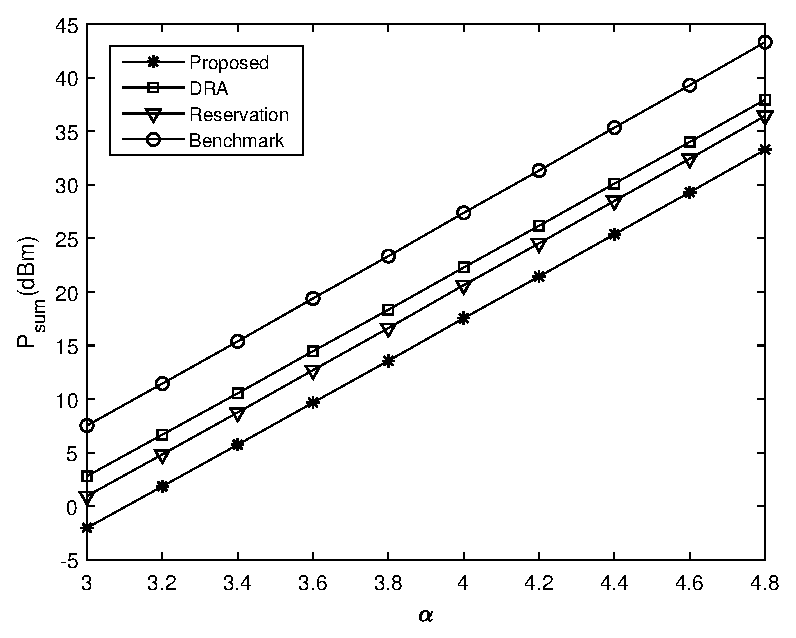
\includegraphics[width=3.6in]{P_alpha.eps}
	\caption{Total transmit power $P_{sum}$ at the six MVNOs versus the path-loss decay factor $\alpha$; performance comparison of different schemes where the total bandwidth is 100MHz and the minimum rate requirement $R_{min}$ is 1Mbps.}
\end{figure}
In Fig. 2, we present the total transmit power $P_{sum}$ comparison of different schemes for different path-loss decay factors $\alpha$ where the total bandwidth is 100MHz and the minimum rate requirement $R_{min}$ is 1Mbps. Note that $P_{sum}$ is defined as the total transmit power at the six MVNOs during the second stage. In the legend, ``Proposed" denotes our proposed blockchain-based distributed spectrum allocation scheme where spectrum and power allocation factors are optimized during both two stages. ``DRA" denotes the dynamic resource allocation scheme where the spectrum and power allocation factors are only optimized during the second stage and the spectrum is equally allocated during the first stage. ``Reservation" denotes the scheme that the spectrum and power allocation factors are only optimized during the first stage and the spectrum is equally allocated during the second stage. ``Benchmark" denotes the scheme that the spectrum is equally allocated both during the first stage and the second stage. It is observed that when the path-loss decay factor $\alpha$ increases, the total transmit power $P_{sum}$ substantially increases for all the schemes. Moreover, our proposed scheme is observed to achieve notably smaller total transmit power than the others schemes, which demonstrates the effectiveness of our proposed spectrum leasing and power allocation scheme.


\begin{figure}
	\centering
	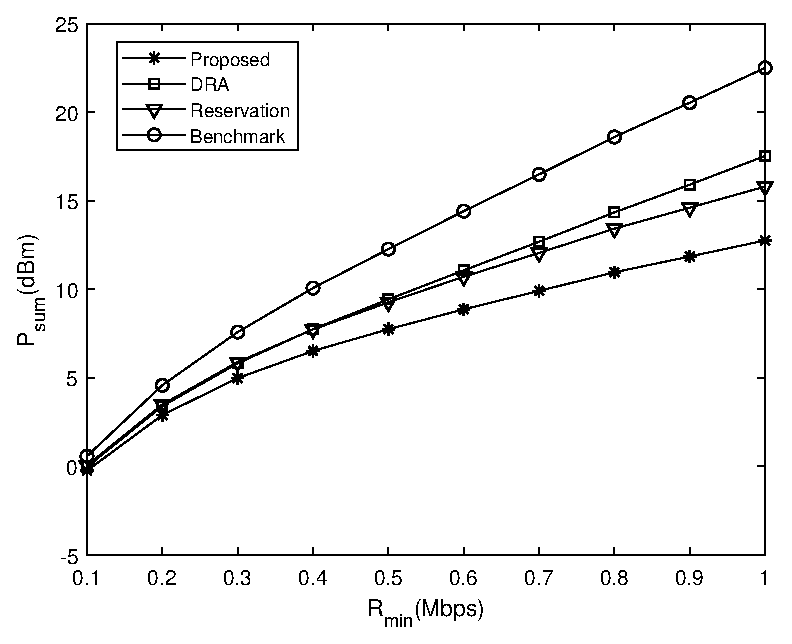
\includegraphics[width=3.6in]{P_rmin.eps}
	\caption{Total transmit power $P_{sum}$ at the six MVNOs versus the minimum rate requirement at MUs; performance comparison of different schemes where the total bandwidth is 100MHz and the path-loss decay factor is 3.76.}
\end{figure}

In Fig. 3, we present the total transmit power $P_{sum}$ comparison of different schemes for different minimum rate requirements $R_{min}$ where the total bandwidth is 100MHz and the path-loss decay factor is 3.76. Here, we assume that $\bar{R}_i = \tilde{R}_i= R_{min}, \forall i$. From Fig. 3, it is observed that as the minimum rate requirement constraint $R_{min}$ becomes more stringent, substantially more total transmit power $P_{sum}$ is needed at the six MVNOs. In particular, the performance gap between our proposed scheme and the other schemes becomes larger as the minimum rate requirements $R_{min}$ increases.

\begin{figure}
	\centering
	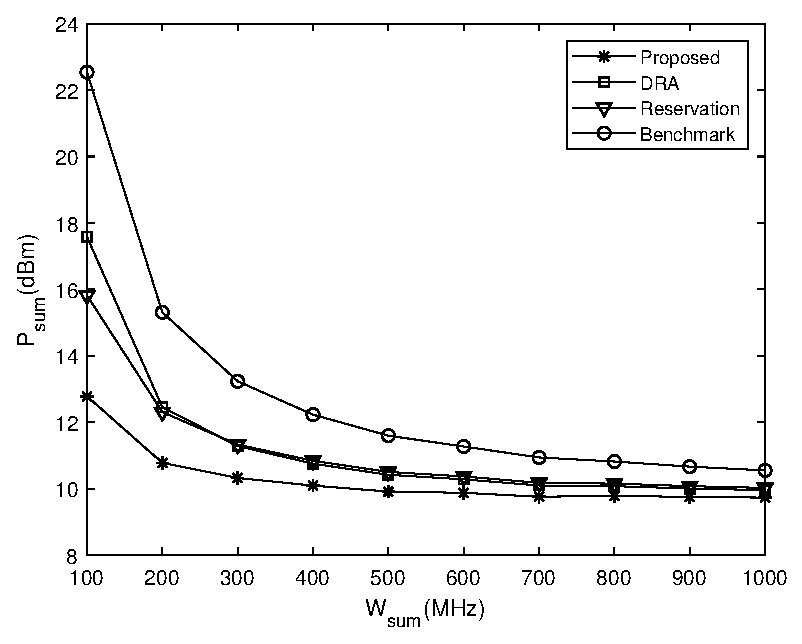
\includegraphics[width=3.6in]{P_wsum.eps}
	\caption{Total transmit power $P_{sum}$ at the six MVNOs versus the total bandwidth $W_{sum}$ owned by the MNO; performance comparison of different schemes where the minimum rate requirement is 1Mbps and the path-loss decay factor is 3.76.}
\end{figure}

In Fig. 4, we present the total transmit power $P_{sum}$ comparison of different schemes for different total bandwidth $W_{sum}$ where the minimum rate requirement is 1Mbps and the path-loss decay factor is 3.76. From Fig. 4, it is observed that as the total bandwidth $W_{sum}$ increases, the total transmit power $P_{sum}$ substantially decreases for all schemes. It is also found that our proposed scheme outperforms the other schemes.

\begin{figure}
	\centering
	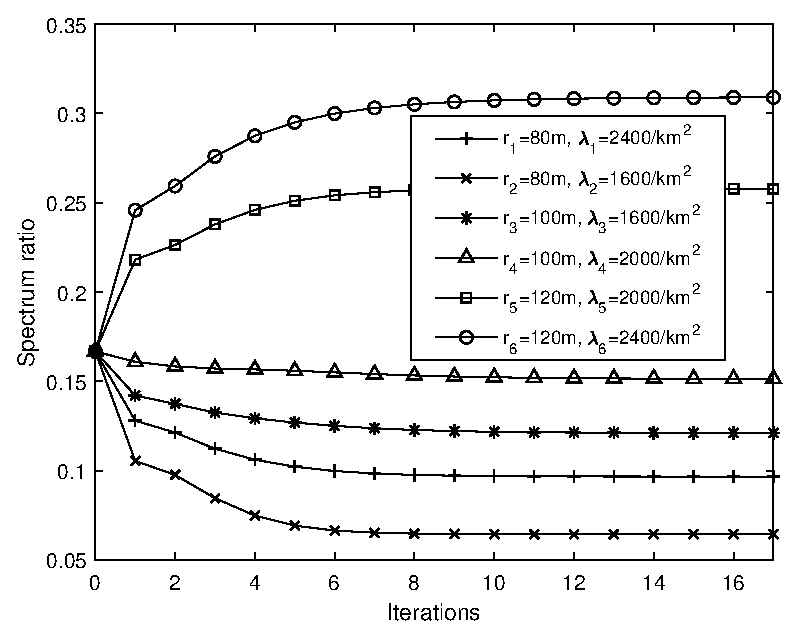
\includegraphics[width=3.6in]{SR_convergence.eps}
	\caption{Spectrum ratio versus the number of iterations where the total bandwidth is 100MHz, the minimum rate requirement is 1Mbps, and the path-loss decay factor is 3.76.}
\end{figure}

In Fig. 5, we present the spectrum ratio occupied by each MVNO for different iteration times where the total bandwidth is 100MHz and the minimum rate requirement is 1Mbps and spectrum ratio is defined as the ratio of the bandwidth occupied by the MVNO to the total bandwidth.  It is found from Fig. 5 that after only 6$\sim$8 iterations, the steady spectrum ratio is achieved. It is also found that both radius and user density in a cell have significant effects on the spectrum ratio. The larger the radius of the cell is configured, the more bandwidth is needed. Likewise, the larger the user density of the cell is configured, the more bandwidth is needed. The main reason behind this phenomenon is that when the user densities of different cells are the same, the channel conditions in cells with large radii are poorer than those with small radii. Thus, more spectrum is needed in large cells for satisfying the QoS of the MUs with poor channel conditions to reduce the total transmit power. Similarly, when the radii of different cells are the same, more spectrum is needed in cells with large user densities than whose with small user densities to meet the QoS constraints.

In Fig. 6, we present the spectrum ratio occupied by each MVNO for different path-loss decay factors, $\alpha$, where the total bandwidth is 100MHz and the minimum rate requirement is 1Mbps. For simplicity, the MVNO with above-average spectrum value is denoted as ``LMVNO" and the MVNO with below-average spectrum value is denoted as ``SMVNO". From Fig. 6, it is observed that the MNO allocates more spectrum to LMVNOs and less spectrum to SMVNOs as $\alpha$ increases. This is because the number of MUs in LMVNOs with poor channel conditions is larger than in SMVNOs and those MUs in LMVNOs with poor channel conditions are more sensitive to the path-loss decay factor $\alpha$. Consequently, more spectrum is needed in LMVNOs to reduce the total transmit power.
 
\begin{figure}
	\centering
	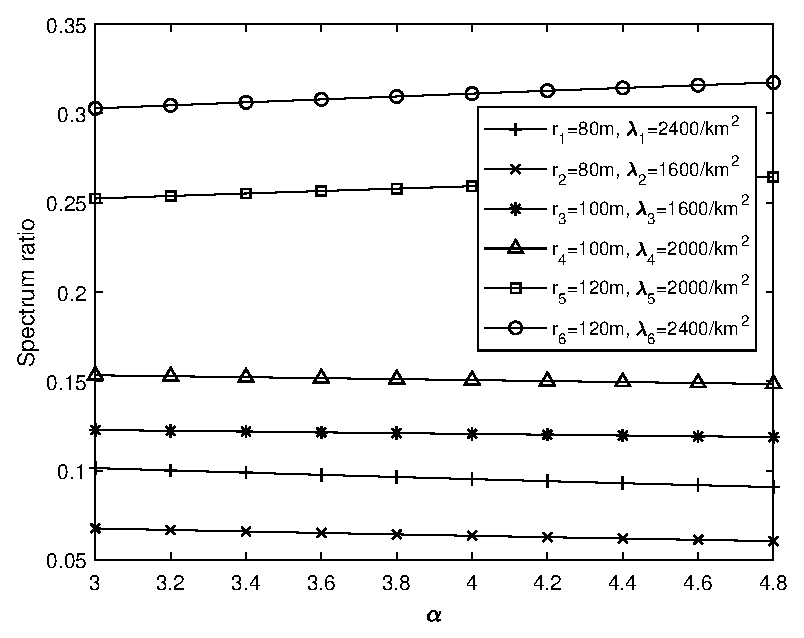
\includegraphics[width=3.6in]{SR_alpha.eps}
	\caption{Spectrum ratio versus the path-loss decay factor $\alpha$ where the minimum rate requirement is 1Mbps and the total bandwidth is 100MHz.}
\end{figure}


\begin{figure}
	\centering
	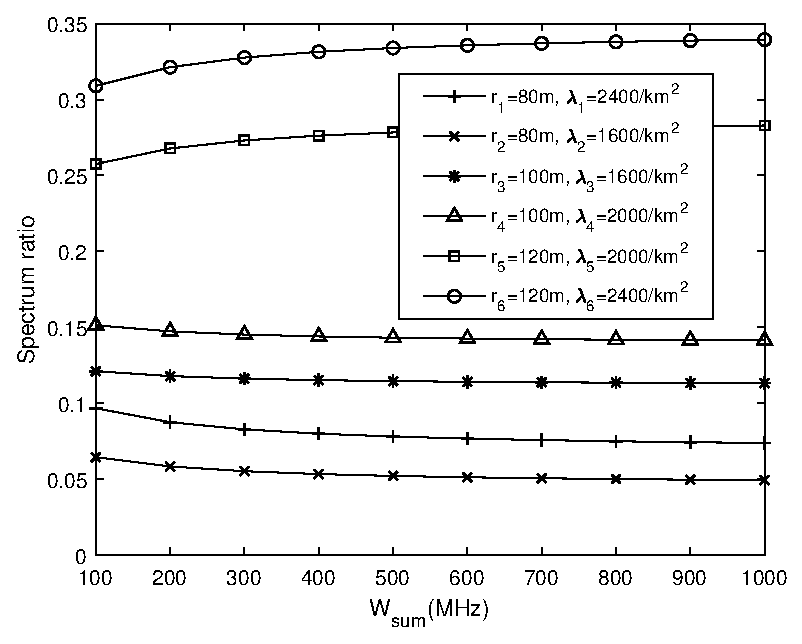
\includegraphics[width=3.6in]{SR_wsum.eps}
	\caption{Spectrum ratio versus the total bandwidth $W_{sum}$ owned by the MNO where the minimum rate requirement is 1Mbps and the path-loss decay factor is 3.76.}
\end{figure}

In Fig. 7, we present the spectrum ratio for different total bandwidths $W_{sum}$ owned by the MNO where the minimum rate requirement is 1Mbps and the path-loss decay factor is 3.76. The results in Fig. 7 show that more spectrum is allocated to SMVNO and less spectrum is allocated to LMVNO as $W_{sum}$ decreases. The reason behind this phenomenon is that from \eqref{q26}, we can observe that the power allocation factor monotonically decreases as the bandwidth increases. Thus, when the bandwidth is in shortage, if we decrease the spectrum allocated to the MUs in SVMNOs, the total transmit power will increase more drastically than in the LVMNOs. Consequently, in order to minimize the total transmit power, more spectrum should be allocated to the MUs in SVMNOs as $W_{sum}$ decreases.

\begin{figure}
	\centering
	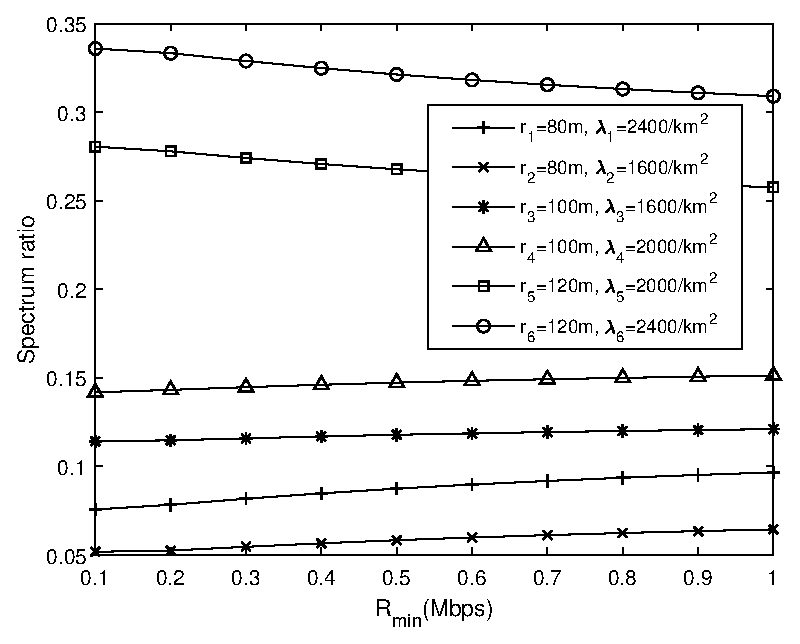
\includegraphics[width=3.6in]{SR_rmin.eps}
	\caption{Spectrum ratio versus the minimum rate requirements $R_{min}$ where the total bandwidth is 100MHz and the path-loss decay factor is 3.76.}
\end{figure}

In Fig. 8, we present the spectrum ratio for different minimum rate requirements, $R_{min}$, where the total bandwidth is 100MHz and the path-loss decay factor is 3.76. From Fig. 8, it is observed that more spectrum is allocated to SMVNO and less spectrum is allocated to LMVNO as $R_{min}$ increases. This is because the transmission rate is monotonically increasing with respect to the bandwidth \eqref{q26}, which means that the bandwidths are more needed when the QoS constraints get more stringent. This coincides with situation that the spectrum is in shortage and thus more spectrum should be allocated to the MUs in SVMNOs as $R_{min}$ increases.
\section{Conclusion}
In this paper, we have investigated a two-stage spectrum allocation problem in the VWN where VMNOs first rent spectrum from the MNO during the first stage and then lease spectrum during the second stage based on the MSs to serve. During the first stage of spectrum leasing, to solve the original optimization problem, a blockchain-based spectrum management scheme combined with ADMM was proposed to obtain the global optimal solutions. During the second stage, we derived the closed-form expressions for the optimization problem. Numerical results have shown that our proposed two-stage spectrum leasing strategies are superior to the other schemes.
\appendices
\section{Proof of Proposition 1}
The CDF of $\left|h_{ij} \right|^2$ is calculated as follows:

\begin{align}
F_{\left|h_{ij} \right|^2} \left(x\right) &= Prob\left(\frac{\left|g_{ij}\right|^2}{1 + d_{ij}^{\alpha}} \leq x \right) \nonumber \\
& = Prob \left(\left|g_{ij}\right|^2 \leq x \left(1 + d_{ij}^\alpha\right)\right) \nonumber \\
& \overset{\left(a\right)}{=} \int_{\mathcal{D}(o_i, r_i)} \frac{1}{\pi r_i^2}\left(1 - e^{-x\left(1 + d_{ij}^{\alpha}\right)}\right) d\Delta S \nonumber\\
& \overset{\left(b\right)}{=} \frac{1}{\pi r_i^2} \int_{0}^{r_i} \int_{-\pi}^{\pi}\left(1 - e^{-x\left(1 + y^{\alpha}\right)}\right)y d \theta d y \nonumber \\
& = \frac{2}{r_i^2}\int_{0}^{r_i} \left(y - ye^{-x\left(1 + y^\alpha\right)}\right) dy \nonumber \\
& = \frac{2}{r_i^2}\int_{0}^{r_i}y dy - \frac{2}{r_i^2}\int_{0}^{r_i} y e^{-x \left(1 + y^\alpha\right)}dy \nonumber \\
& = 1 - \frac{2}{r_i^2}e^{-x} \int_{0}^{r_i}y e^{-xy^{\alpha}}dy
\end{align}
where $\left(a\right)$ follows from the CDF of the exponential random variable $\left|g_{ij}\right|^2$, $\left(b\right)$ follows by using polar coordinates. Let $t = xy^{\alpha}$, $F_{\left|h_{ij} \right|^2} \left(x\right)$ can be further derived as follows:
\begin{align}
F_{\left|h_{ij} \right|^2} \left(x\right) &= 1 - \frac{2}{r_i^2}e^{-x} \int_{0}^{x r_i^{\alpha}} t^{\frac{1}{\alpha}} x^{-\frac{1}{\alpha}}e^{-t} d\left(t^{\frac{1}{\alpha}} x^{-\frac{1}{\alpha}}\right) \nonumber \\
& = 1 - \frac{1}{\alpha} \frac{2}{r_i^2} x^{-\frac{2}{\alpha}} e^{-x} \int_{0}^{x r_i^{\alpha}} t^{\frac{2}{\alpha} - 1}e^{-t} dt \nonumber \\
& = 1 - \frac{2}{\alpha} \left(x r_i^{\alpha}\right) ^{-\frac{2}{\alpha}} \gamma\left(\frac{2}{\alpha}, xr_i^{\alpha}\right)e^{-x} \nonumber \\
& \overset{\left(c\right)}{=} 1 - M\left(\frac{2}{\alpha}, 1 + \frac{2}{\alpha}, -xr_i^{\alpha}\right)e^{-x}
\end{align}
where $\gamma\left(s,x\right) = \int_{0}^{x}t^{s-1}e^{-t}dt$ denotes the lower incomplete gamma function, $M\left(\cdot,\cdot,\cdot\right)$ denotes the Kummer's function \cite{MAbramowitz}, $\left(c\right)$ follows from $\gamma\left(s,x\right) = s^{-1} x^s M\left(s,1+s,-x\right)$ \cite[6.5.12]{MAbramowitz}. Thus the proof is completed. 

\section{Proof of Proposition 2}
The Lagrangian of problem \eqref{eq28} is given by
\begin{align}
\mathcal{L}\left(b_{ij}, \mu\right) &=  \sum\limits_{i = 1}^{N_i} \frac{b_{ij}n_0}{\left|h_{ij}\right|^2}\left(2^{\frac{\tilde{R}_i}{b_{ij}}} - 1\right) + \mu\left(\sum_{j = 1}^{N_i}b_{ij} - w_i\right) \nonumber \\ 
& \overset{\left(h\right)}{=} \sum\limits_{i = 1}^{N_i} \frac{b_{ij}n_0}{\left|h_{ij}\right|^2}\left(e^{\frac{\hat{R}_i}{b_{ij}}} - 1\right) + \mu\left(\sum_{j = 1}^{N_i}b_{ij} - w_i\right) 
\end{align}
where $\mu \geq 0$ denotes the Lagrange multiplier associated with the constraint \eqref{q28b}. $\left(h\right)$ follows from $\hat{R}_i = \tilde{R}_i \ln2$. Thus, the dual function of problem \eqref{eq28} is given by
\begin{align}
\mathcal{G}\left(\mu\right) = \min_{b_{ij}\geq 0} \mathcal{L}\left(b_{ij},\mu\right)
\end{align}

It can be seen from problem \eqref{eq28} that there exist a set of $b_{ij}$ with $b_{ij} > 0$, satisfying $\sum\limits_{j = 1}^{N_i} b_{ij} < w_i, \forall j$. Thus, thanks to the Slater's condition, strong duality for problem \eqref{eq28} holds. The Karush-Kuhn-Tucker (KKT) conditions which are both necessary and 	sufficient for the  global optimality of problem \eqref{eq28} are given by
\begin{align}
\frac{\partial \mathcal{L}\left({b_{ij}^\star}, \mu^\star\right)}{\partial b_{ij}} &= 0 \label{q36} \\
\mu^\star\left(\sum\limits_{j = 1}^{N_i}b_{ij}^\star - w_i\right) &= 0 \label{q37} \\
\sum\limits_{j = 1}^{N_i}b_{ij}^\star - w_i & \leq 0 \label{q38}
\end{align} 
where $b_{ij}^\star$ and $\mu^\star$ denote the optimal primal and dual solutions of problem \eqref{eq28}, respectively. It can be easily verified that $\sum\limits_{j = 1}^{N_i} b_{ij}^\star = w_i$ must hold for problem \eqref{eq28}. Thus, from \eqref{q37}, we have $\mu^\star > 0$. From \eqref{q36}, it follows that 
\begin{align}
\frac{\partial \mathcal{L} \left(b_{ij}^\star, \mu^\star \right)}{\partial b_{ij}} &= \frac{n_0}{\left|h_{ij}\right|^2} \left(e^{\frac{\hat{R}}{b_{ij}^\star}} -  \frac{\hat{R}_i}{b_{ij}^\star} e^{\frac{\hat{R}_i}{b_{ij}^\star}} - 1\right) + \mu^\star \nonumber \\
& =  \frac{n_0}{\left|h_{ij}\right|^2}\left(\left(1 - \frac{\hat{R}_i}{b_{ij}^\star}\right)e^{\frac{\hat{R}_i}{b_{ij}^\star} - 1}e - 1\right) + \mu^\star \nonumber \\
& = 0. \label{q39}
\end{align}
From \eqref{q39}, we have
\begin{align}
\left(\frac{\hat{R}_i}{b_{ij}^\star} - 1\right) e^{\frac{\hat{R}}{b_{ij}^\star} - 1} = \frac{\mu^\star \left|h_{ij}\right|^2 - n_0}{n_0 e},
\end{align}
according to the definition of Lambert $\mathcal{W}$ function, we can obtain the optimal $b_{ij}^\star$ as follows:
\begin{align}
b_{ij}^\star = \frac{\hat{R}_i}{1 + \mathcal{W}_0\left(\frac{\mu^\star \left|h_{ij}\right|^2 - n_0}{n_0 e}\right)} \label{q41},
\end{align}
where $\mathcal{W}_0\left(\phi\right)$ is the branch satisfying $\mathcal{W}\left(\phi\right) \geq -1$, $\mathcal{W}$ denotes the Lambert $\mathcal{W}$ function of $\phi$ \cite{RMCorless} and the optimal $\mu^\star$ can be obtained via a 1-D bisection search over $\left[\mu_{min}, \mu_{max}\right]$ with $\mu_{min} $ and $\mu_{max}$ derived as follows.

Denote the maximum and minimum channel gains among $N_i$ users in the $i$-th cell as $h_{max}$ and $h_{min}$  , respectively. Thus, we have
\begin{align}
h_{min} \leq \left|h_{ij}\right|^2 \leq h_{max}.
\end{align}
Since $\mathcal{W}_0\left(x\right)$ is monotonically increasing when $x \geq 0$, it follows that
\begin{align}
&\mathcal{W}_0\left(\frac{\mu^\star h_{min} - n_0}{n_0e}\right) \nonumber \\ & \leq  \mathcal{W}_0 \left(\frac{\mu^\star\left|h_{ij}\right|^2 - n_0}{n_0e}\right) \leq  \mathcal{W}_0\left(\frac{\mu^\star h_{max} - n_0}{n_0e}\right)
\end{align}
Combined with \eqref{q41}, the above inequality can be reformulated as
\begin{align}
\frac{\hat{R}_i}{1 + \mathcal{W}_0\left(\frac{\mu^\star h_{max} - n_0}{n_0e}\right)} \leq b_{ij}^\star \leq \frac{\hat{R}_i}{1 + \mathcal{W}_0\left(\frac{\mu^\star h_{min} - n_0}{n_0e}\right)} \label{q44}
\end{align}
After adding each term in \eqref{q44} from $j = 1$ to $j = N_i$, we can obtain the following inequality
\begin{align}
\frac{N_i\hat{R}_i}{1 + \mathcal{W}_0\left(\frac{\mu^\star h_{max} - n_0}{n_0e}\right)} \leq w_{i} \leq \frac{N_i\hat{R}_i}{1 + \mathcal{W}_0\left(\frac{\mu^\star h_{min} - n_0}{n_0e}\right)} 
\end{align}
Finally, we have
\begin{align}
\mu_{min} \leq \mu^\star \leq \mu_{max}
\end{align}
where 
\begin{align}
\mu_{min} &= \frac{n_0\left(\frac{N_i\hat{R}_i}{w_i} - 1\right)e^{\frac{N_i\hat{R}_i}{w_i}} + n_0}{h_{max}}  \\
\mu_{max} & = \frac{n_0\left(\frac{N_i\hat{R}_i}{w_i} - 1\right)e^{\frac{N_i\hat{R}_i}{w_i} } + n_0}{h_{min}}
\end{align}
The proof is completed.
 
\begin{thebibliography}{1}	
\bibitem{NPanwar} N. Panwar, S. Sharma, and A. K. Singh, ``A survey on 5G: The
next generation of mobile communication," \emph{Phys. Commun.}, vol. 18, pp. 64-84, Mar. 2016.	
	
\bibitem{NAlFalahy} N. Al-Falahy and O. Y. Alani, ``Technologies for 5G networks:
Challenges and opportunities," \emph{IT Prof.}, vol. 19, no. 1, pp. 12-20, Jan./Feb. 2017.	

\bibitem{AYDing} A. Y. Ding and M. Janssen, ``Opportunities for Applications Using 5G Networks: Requirements, Challenges, and Outlook,” in \emph{Proc. of the Seventh International Conference on Telecommunications and Remote Sensing(ICTRS 2018)}, 2018, pp. 27-34.

\bibitem{JRosenworcel} J. Rosenworcel, ``Commissioner Rosenworcel Remarks at Mobile World Congress Americas, Los Angeles, CA," Federal Communications Commission, Sep. 2018. [Online]. Available: https://docs.fcc.gov/public/attachments/DOC-354091A1.pdf.
	
\bibitem{CLiang} C. Liang and F. R. Yu, ``Wireless network virtualization: A survey, some research issues and challenges,” \emph{IEEE Comm. Surveys Tutorials}, vol. 17, pp. 358-380, Firstquarter 2015.

\bibitem{LZhao}L. Zhao, M. Li, Y. Zaki, A. Timm-Giel and C. Gorg, ``LTE virtualization:
From theoretical gain to practical solution," \emph{in Proc. International Teletraffic Congress (ITC)}, pp. 71-78, Sep. 2011.


\bibitem{3GPP}3GPP TR 22.852, ``Study on Radio Access Network (RAN) sharing enhancements," Jun. 2013.

\bibitem{RKokku} R. Kokku, R. Mahindra, H. Zhang, and S. Rangarajan, ``NVS: A substrate for virtualizing wireless resources in cellular networks," \emph{IEEE/ACM Trans. Netw.}, vol. 20, no. 5, pp. 1333-1346, Oct. 2012.

\bibitem{XCostaPerez}X. Costa-Perez, J. Swetina, T. Guo, R. Mahindra, and S. Rangarajan, ``Radio access network virtualization for future mobile carrier networks," \emph{IEEE Commun. Mag.}, vol. 51, no. 7, pp. 27-35, Jul. 2013.

\bibitem{MIKamel}M. I. Kamel, L. Bao Le, and A. Girard, ``LTE wireless network virtualization: dynamic slicing via flexible scheduling," \emph{in Proc. IEEE VTC Fall}, pp. 1-5, Sept. 2014.

\bibitem{MKalil}M. Kalil, A. Moubayed, A. Shami, and A. Al-Dweik, ``Efficient low-complexity scheduler for wireless resource virtualization," \emph{IEEE Wireless Commun. Letters}, vol. 5, no. 1, pp. 56-59, Feb 2016.
	
\bibitem{YXZhang1}Y. Zhang, S. Bi, and Y. J. A. Zhang, ``A two-stage spectrum leasing optimization framework for virtual mobile network operators," in \emph{IEEE Int. Conf. on Commun. Syst. (ICCS)}, Dec. 2016, pp. 1-6.

\bibitem{YXZhang2}Y. Zhang, S. Bi, and Y. J. A. Zhang, ``Joint Spectrum Reservation and On-demand Request for Mobile Virtual Network Operators," \emph{IEEE Trans. Commun.}, vol. 66, no. 7, pp. 2966-2977, July, 2018.	

\bibitem{FBltr}F. Beltr{\'a}n and M. Massaro, ``Spectrum management for 5G: assignment methods for spectrum sharing," in \emph{29th European Regional Conference of the International Telecommunications Society}, 2018.

\bibitem{SNakamoto}S. Nakamoto, ``Bitcoin: A peer-to-peer electronic cash system," 2008. [Online]. Available: https://bitcoin.org/bitcoin.pdf

\bibitem{KGai}K. Gai, K.-K. R. Choo, and L. Zhu, ``Blockchain-Enabled Reengineering of Cloud Datacenters," \emph{IEEE Cloud Comput.}, vol. 5, no. 6, pp. 21-25, Nov. 2018.

\bibitem{PKSharma}P. K. Sharma, S. Singh, Y. S. Jeong, and J. H. Park, ``DistBlockNet: A Distributed Blockchains-Based Secure SDN Architecture for IoT Networks," \emph{IEEE Commun. Mag.}, vol. 55, no. 9, pp. 78-85, 2017.

\bibitem{ZXiong}Z. Xiong, S. Feng, W. Wang, D. Niyato, P. Wang, and Z. Han, ``Cloud/Fog Computing Resource Management and Pricing for Blockchain Networks," \emph{IEEE Internet Things J.}, pp. 1-1, 2018.

\bibitem{DBRawat}D. B. Rawat and A. Alshaikhi, ``Leveraging Distributed Blockchain-based Scheme for Wireless Network Virtualization with Security and QoS Constraints," in \emph{2018 International Conference on Computing, Networking and Communications (ICNC 2018)}, 2018, pp. 332-336.

\bibitem{E. Munsing}E. M\"{u}nsing, J. Mather, and S. Moura, ``Blockchains for decentralized optimization of energy resources in microgrid networks,’’ in \emph{Proc. IEEE
Conf. Control Technol. Appl. (CCTA)}, Aug. 2017, pp. 2164-2171.

\bibitem{KKotobi}K. Kotobi and S. G. Bilen, ``Secure Blockchains for Dynamic Spectrum Access: A Decentralized Database in Moving Cognitive Radio Networks Enhances Security and User Access," \emph{IEEE Veh. Technol. Mag.}, vol. 13, no. 1, pp. 32-39, Mar. 2018.
	
\bibitem{JGDForney}J. G. D. Forney and G. Ungerboeck, ``Modulation and coding for linear gaussian channels," \emph{IEEE Trans. Inf. Theory}, vol. 44, no. 6, pp. 2384-2415, Oct. 1998.

\bibitem{MAbramowitz}M. Abramowitz and I. A. Stegun, Handbook of mathematical functions: with formulas, graphs, and mathematical tables, vol. 55. \emph{Courier Corporation}, 1965.

\bibitem{JSBall}J. S. Ball, ``Half-range generalized Hermite polynomials and the related Gaussian quadratures," \emph{SIAM J. Numer. Anal.}, vol. 40, no. 6, pp. 2311-2317, 2002.

\bibitem{NMSteen}N. M. Steen, G. D. Byrne, and E. M. Gelbard, ``Gaussian quadratures for the integrals $\int_{0}^{\infty} e^{-x^2}f\left(x\right) dx$ and $\int_{0}^{b}e^{-x^2}f\left(x\right)dx$," \emph{Math. Comput.}, vol. 23, no. 107, pp. 661-671, 1969.

\bibitem{SBoyd1}M. Grant and S. Boyd, \emph{CVX: MATLAB Software for Disciplined Convex Programming.} Version 2.1, 2016, available: http://cvxr.com/cvx.

\bibitem{SBoyd2}S. Boyd, N. Parikh, E. Chu, B. Peleato, and J. Eckstein, ``Distributed optimization and statistical learning via the alternating direction method of multipliers," \emph{Found. Trends in Mach. Learn.}, vol. 3, no. 1, pp. 1-122, Jan. 2011.

\bibitem{EChen}E. Chen and M. Tao, ``ADMM-based fast algorithm for multi-group multicast beamforming in large-scale wireless systems," \emph{IEEE Trans. Commun.}, vol. 65, no. 6, pp. 2685-2698, Jun. 2017.

\bibitem{SBoyd3}S. Boyd and L. Vandenberghe, Convex Optimization. Cambridge, U.K.: Cambridge Univ. Press, 2004.

\bibitem{JDuchi}J. Duchi, S.Shalev-Shwartz, Y. Singer, and
T. Chandra, ``Efficient projections onto
the $l_1$-ball for learning in high dimensions," in \emph{Proc. 25th Int. Conf}. Mach. Learn., 2008,
DOI: 10.1145/1390156.1390191.

\bibitem{RMCorless}R. M. Corless, G. H. Gonnet, D. E. G. Hare, D. J. Jeffrey, and D. E.
Knuth, ``On the Lambert W function," \emph{Adv. Comput. Math.}, vol. 5, pp. 329-359, 1996.
\end{thebibliography}


\end{document}
